\begin{figure}
	\centering
	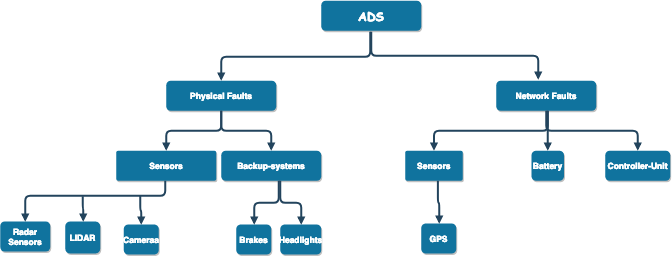
\includegraphics[width=1.0\linewidth]{Fault-model1}
	\caption[Fault-model for ADS]{This shows a general fault model of Autonomous Driving Systems. We have kept it generic enough to be considered for different Autonomous systems. However, our work is oriented towards aunomous cars.}
	\label{fig:fault-model1}
\end{figure}
\section{Related Work} 

Reliability and safety of individual components in ADS have been previously studied. Li et al.~\cite{guanpeng17sc} studied the impact of soft errors on DNN using Fault injections on hardware accelerators and proposed solutions for making DNNs more resilient. Using Fault injections for testing reliability of system has inherent disadvantage that for complex systems like DNNs a huge number of FI are required to get statistically meaningful insights, moreover the coverage that FI provides is also dependent on the input used for FI, so in case of DNN where the input has a diverse range, performing FI to get meaningful resilience profile of a DNN sub-system of an ADS can be quite resource intensive, otherwise some corner case may be missed during the analysis. Keeping these things in mind Pi et al.~\cite{kexin17sosp} introduced DeepXplore, which tests deep learning systems in a systematic way by finding the inputs for DL systems, that will result in mismatch in output for different DL systems that provide same functionality. In this way corner cases that are not captured by regular testing and training cycle in neural networks are found thus exposing erroneous behavior of the system without a significant overhead of finding corner cases manually. DeepXplore also finds input that maximize the fraction of neurons activated when tested, thus increasing the tests coverage of DNNs. DeepXplore can provide a good defense against vulnerabilities and erroneous behaviors in DNN part of ADS but for overall reliability of the program other components of the system also need to be analyzed.

Jha et al.~\cite{jha18dsn} developed AVFI which is a fault injector that performs resilience assessment of complete autonomous vehicle(AV) systems. AVFI inject faults in without any systematic approach in AV system which consists of CARLA simulator and a driving agent which performs the control actions. AVFI can inject hardware faults (modeling soft errors), data faults (modeling error in sensor values), timing faults and machine learning faults (errors leading to wrong prediction). Jha et al.~\cite{jha18art} developed Kayotee which is a FI based tool to inject faults in an ADS (similar to AVFI) and then classifying errors and safety violations impacting the reliability of autonomous vehicles. Kayotee injects faults in both hardware and software components of proprietary Nvidia DriveWorks platform, in a closed looped environment and then error propagation and masking characteristics of the ADS compute stack are evaluated using a predefined ontology model.Kayotee and AVFI provides a holistic view of the system but its  fault coverage is also limited, as only those errors can be studied which have been simulated using FI. As whole system is taken into consideration during holistic analysis, trying to increase the test coverage using FI can lead to state space explosion.  